\renewcommand{\thefigure}{\arabic{section}.\arabic{subsection}.\arabic{figure}}

\begin{enumerate}
		\item[\textbf{Ques.}] 
		{ Two sides AB and BC and median AM of one
		triangle ABC are respectively equal to sides PQ
		and QR and median PN of $\Delta$ PQR.Show that:}

	\begin{enumerate}
		\item$\Delta$ ABM $\cong$ $\Delta$ PQN  
		\item$\Delta$ ABC $\cong$ $\Delta$ PQR
	\end{enumerate}
	
	\item [\textbf{Ans.}]

	\begin{enumerate}
		\item Let assume we have two triangles as follows$\to$\\
		
		\begin{figure}[!htb]
			%\begin{minipage}{0.48\textwidth}
				\centering
				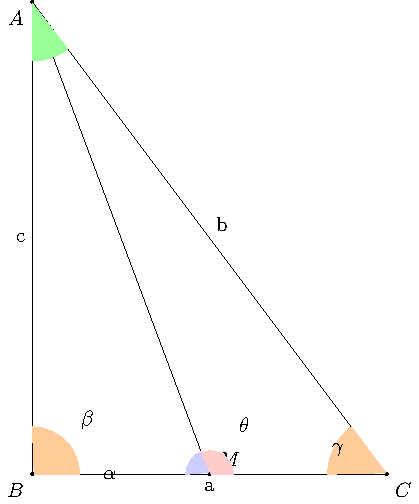
\includegraphics[width=2.0in]{./figures/congurentpicabc.pdf}
				\caption{$\Delta$ ABC}
				\label{fig:triangle}
	    	%\end{minipage}
	    \end{figure}
        \begin{lstlisting}
       ./figures/congurentpicabc.pdf
        \end{lstlisting}
	    	%\hfill
	   	\begin{figure}
	    	%\begin{minipage}{0.48\textwidth}
				\centering
				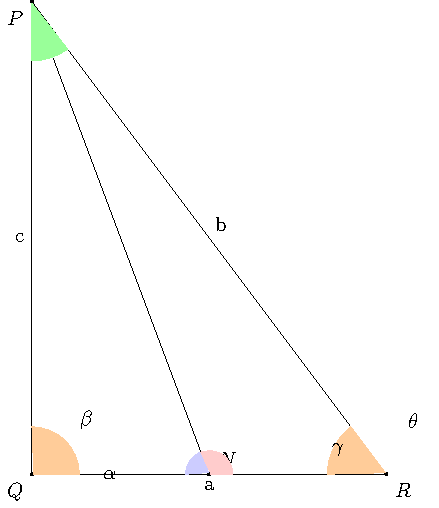
\includegraphics[width=2.0in]{./figures/congurentpicabc2.pdf}
				\caption{$\Delta$ PQR }
				\label{fig:triangle2}
	   	 	%\end{minipage}	
    	\end{figure}
    	\begin{lstlisting}
    ./figures/congurentpicabc2.pdf
    	\end{lstlisting}
    

		given that $\to$\\
		\begin{align}
			AB = PQ\\
			AM = PN\\
			BC = QR	
		\end{align}
	
		from equation $\left(1.0.3\right)$...
	
		\begin{align}
			\frac{BC}{2} = \frac{QR}{2} \\
			BM = QN
		\end{align}

		from fig $\left[1.0.1\right]$ and $\left[1.0.2\right]$ ...

		\begin{align}
	 		AB = PQ\\
	 		AM = PN\\
	 		BM = QN\\
			\implies  \Delta ABM \cong \Delta PQN
		\end{align}
	
		\item
		given that $\to$\\
		\begin{align}
			AM = PN
		\end{align}
	
		from equation $\left(1.0.3\right)$...
	
		\begin{align}
			\frac{BC}{2} = \frac{QR}{2} \\
			MC = NR
		\end{align}
	
	
		from equation $\left(1.0.9\right)$...
		\begin{align}
			\Delta ABM \cong \Delta PQN 
			\\
			\implies \angle AMB = \angle PNQ
			\\
			180 - \angle AMB = 180 -  \angle PNQ
			\\
			\angle AMC = \angle PNR
		\end{align}
	
		from equation $\left(1.0.10\right)$,$\left(1.0.12\right)$ and $\left(1.0.16\right)$...
		\begin{align}
			AM = PN
			\\
			MC = NR
			\\
			\angle AMC = \angle PNR
			\\
			\implies  \Delta AMC \cong \Delta PNR
			\\
			\implies AC = PR
		\end{align}
	
		from equation $\left(1.0.1\right)$,$\left(1.0.3\right)$ and $\left(1.0.21\right)$...
		
		\begin{align}
			AB = PQ\\
			BC = QR\\
			AC = QR\\
			\implies  \Delta ABC \cong \Delta PQR
		\end{align}
	
	\end{enumerate}
	
\end{enumerate}
